
	
	In order to try the reverse control from the Google Glass to the electrovalves we made different kind of experiments.
	
	\section{LED Experiments}
	 First of all we tried the circuit on a breadboard using LEDs instead of electrovalves. The aim of this step is to demonstrate that the firmware running on the Beaglebone Black, the Java code running on the Google Glass and the Python code running on the Google App Engine (used to store the information about the electrovalves status) work well.\\
	Moreover the LED and the electrovalve have basically the same behavior so, if everything works well with the LEDs, there are all the reasons to believe that everything is going to work well with the electrovalves, too.\\
	
	The circuit that actually drives the LEDs is very simple, and it is based on a MOS transistor (\href{http://www.onsemi.com/pub_link/Collateral/BS170-D.PDF}{\textit{BS170}}) used as a switch voltage-controlled, as shown in (Fig.\ref{Fig:driverLED}).
	
	\begin{figure}[h]
		\centering
		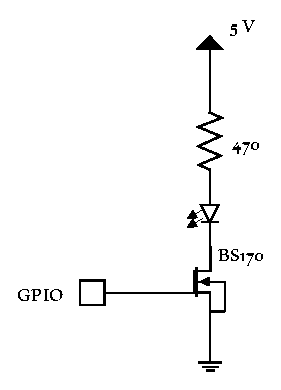
\includegraphics[]{Driver/driverLED}
		\caption{Driver for LED}
		\label{Fig:driverLED}
	\end{figure}
	
	The (Fig.\ref{Fig:circuitLED}) shows the circuit used for this step of testing. As can be seen the number of LEDs used is eight, the same number of electrovalves that can be driven from this system.\\
	In order to test all of them we made 2 different kind of trials:
	\begin{enumerate}
		\item \textit{In order turning on\&off}, first all the LEDs are turned on starting from the first one (on the top right corner) to the last one (on the bottom left corner). Then the LEDs are turned off following the same order.\\The result of this can bee watched in  \href{http://youtu.be/iYeAMpxM9uI}{\textbf{this}} video.
		\item \textit{Out of order turning on\&off}, in this trial, like before, all the LEDs start from a condition where all of them are off and then we turned on and off all the LEDs, but in this case following a random order.\\ The result of this can bee watched in  \href{http://youtu.be/mIoylW334Ck}{\textbf{this}} video.
	\end{enumerate}
	
	
	\begin{figure}[h]
		\centering
		\includegraphics[scale=.21]{Experiments/ledBoard}
		\caption{LEDs experiments board}
		\label{Fig:circuitLED}
	\end{figure}
	
	
	\section{Electrovalves experiments}
	
	\subsection{Breadboard Phase}
	The (Fig.\ref{Fig:circuitBreadboard}) shows from the top view the circuit used during the second phase of experiment, the one where we started using electrovalves in a real microfluidic application.\\
	On the left side of the figure we can see the conditioning circuits for the temperature sensor (on the top) and pH sensor (on the bottom). While, on the other side, we can see the part of circuit in charge to drive the electrovalves.\\
	In this last one we are going to focus for now. Each electrovalve is driven by the circuit shown in (Fig.\ref{Fig:driverEV}).
	\clearpage
	
	
	
	As you can see, this circuit is pretty close to the one of (Fig.\ref{Fig:driverLED}), indeed the only difference is given by freewheeling diode, mandatory because of inductive behavior of electrovalve's solenoid.
	
	\begin{figure}[h]
		\centering
		\includegraphics[scale=.14]{circuitBreadboard}
		\caption{Circuit mounted on breadboard top view}
		\label{Fig:circuitBreadboard}
	\end{figure}
	
	
	The result of the experiments with electrovalves in a real microfluidic case can bee watched in  \href{https://www.youtube.com/watch?v=CavCVnD2P1k}{\textbf{this}} video.
	
	\begin{figure}[h]
		\begin{center}
		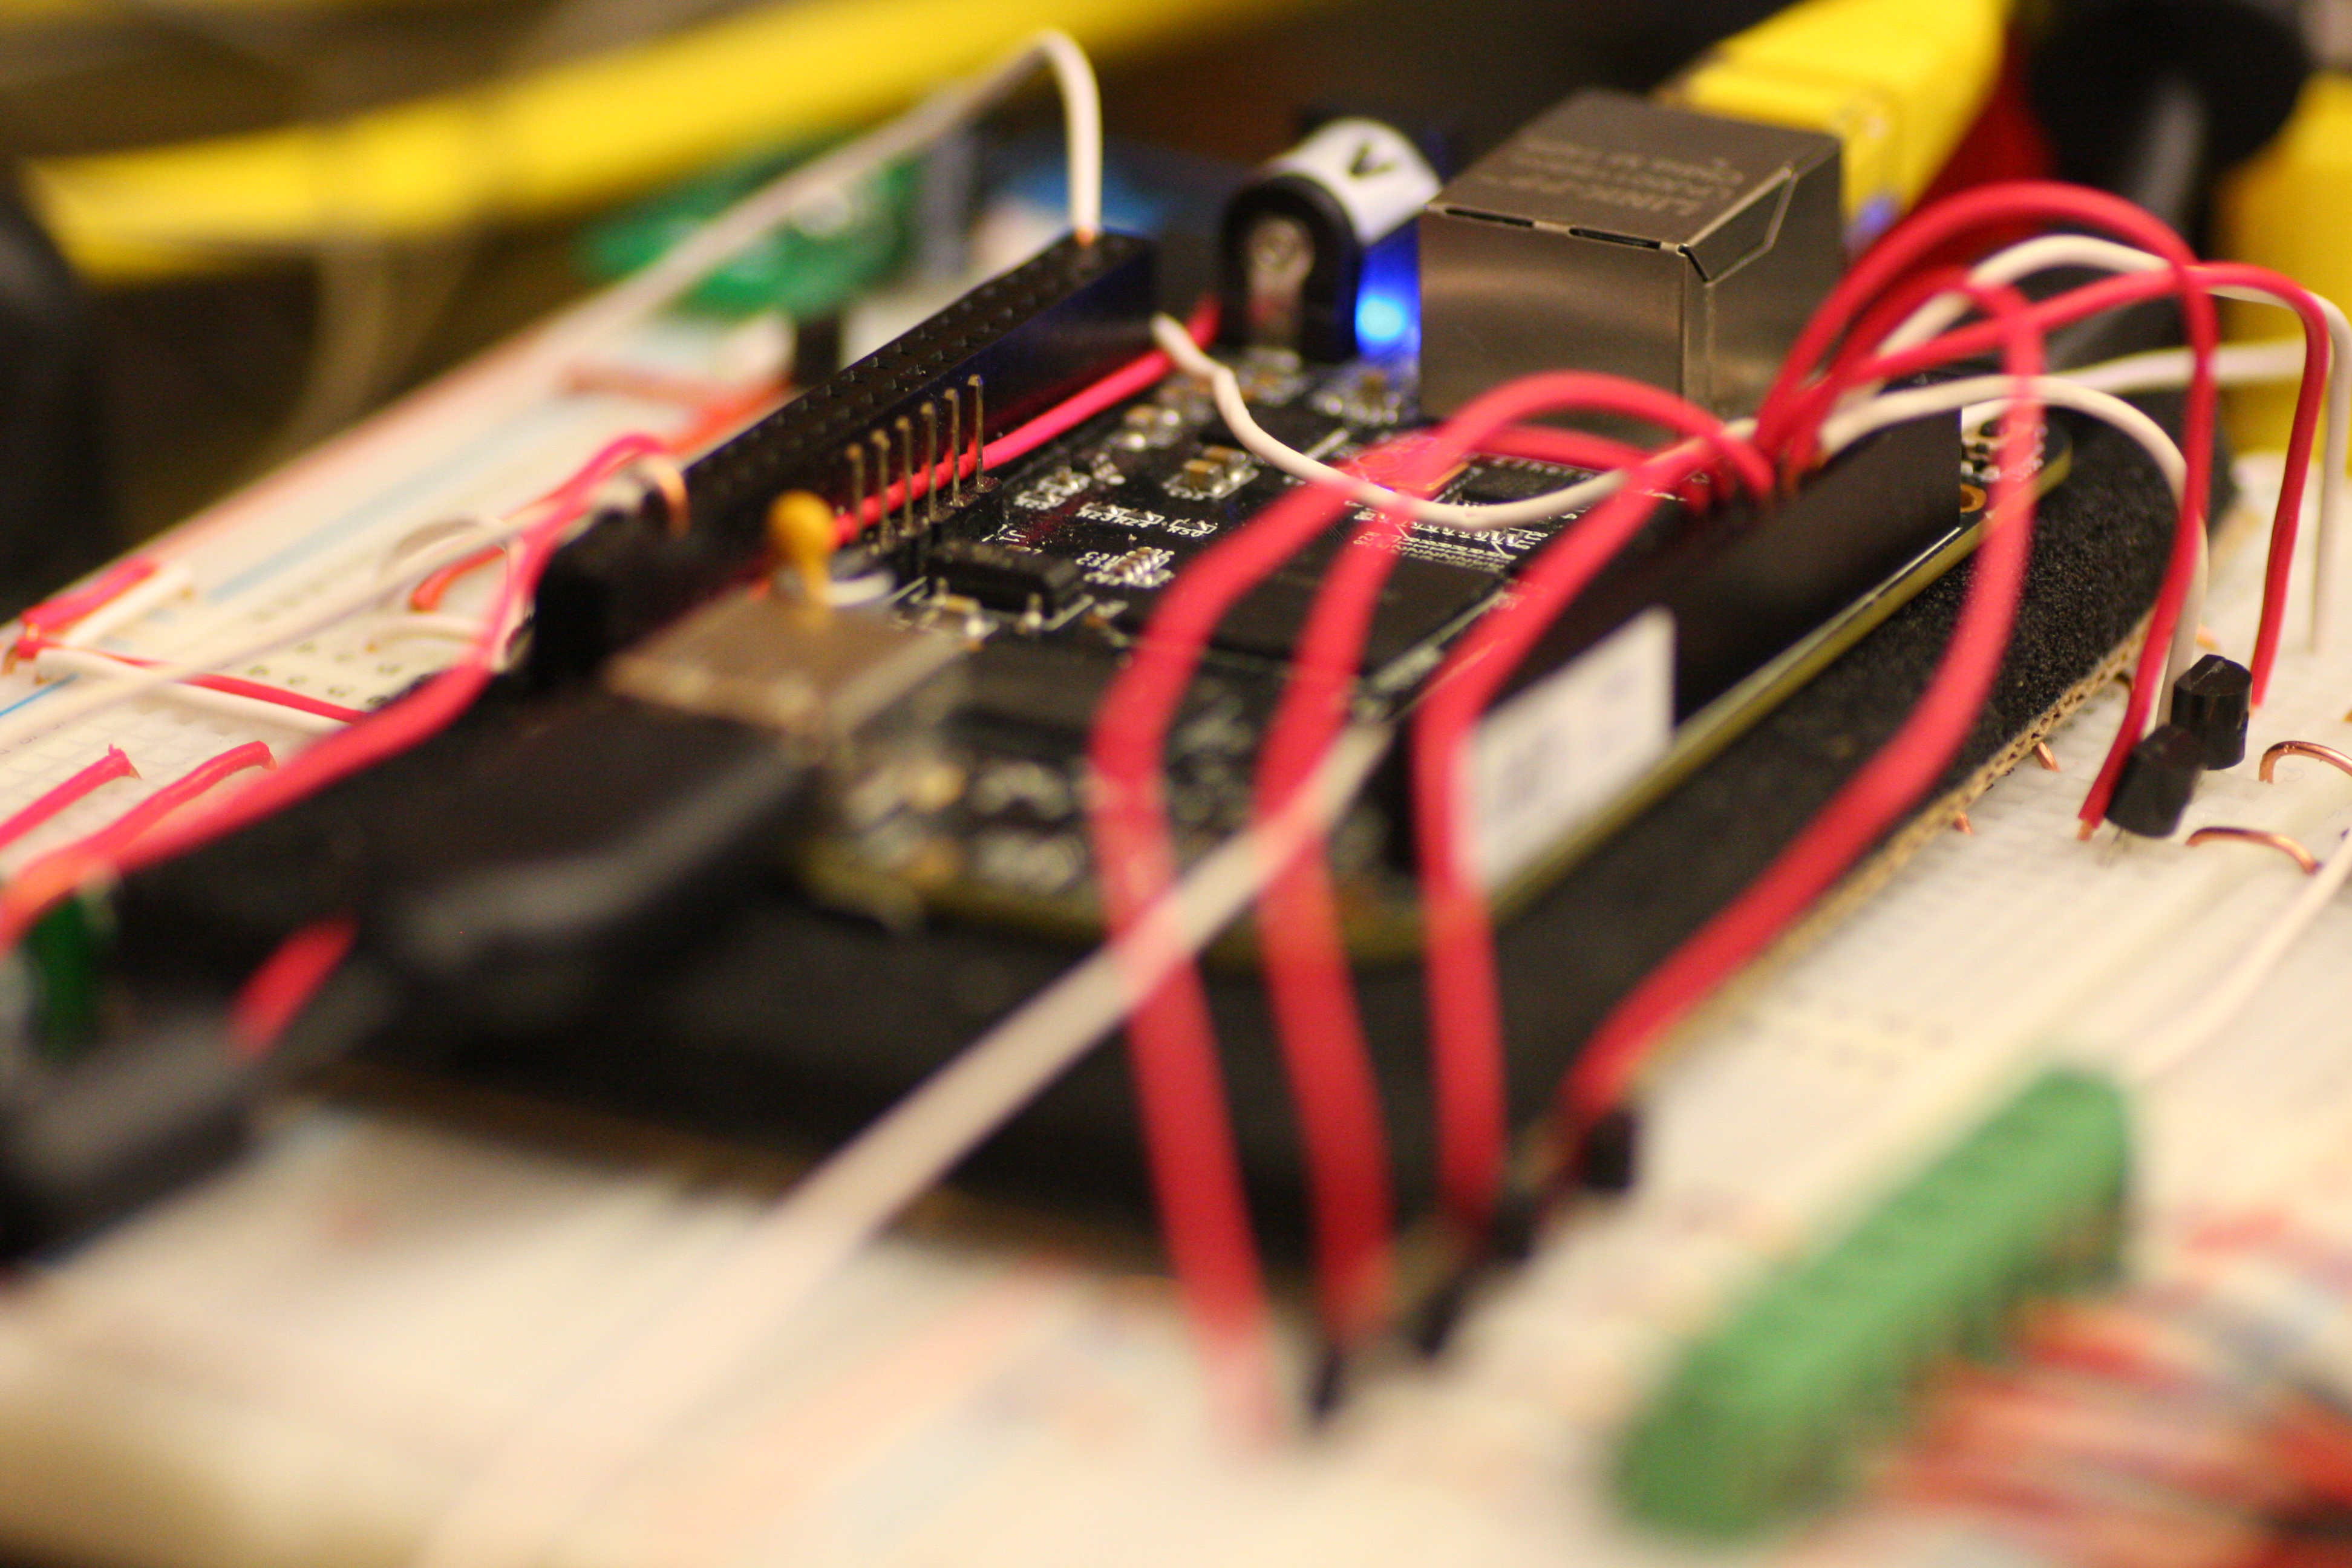
\includegraphics[width=\textwidth]{breadboard}
		\caption{Circuit mounted on breadboard side view}
		\label{Fig:circuitsfumatp}
	\end{center}
	\subsection{PCB Phase}
	
	Finally we replied the last experiment using a PCB (Fig.\ref{fig:PCB}),  designed for this system.\\
	As expected the result of this experiment is the same of the previus step. 
	\end{figure}